\documentclass[ignorenonframetext, hyperref=unicode]{beamer}



\usepackage{cmap}
%\usepackage[T2A]{fontenc}
\usepackage[utf8]{inputenc}
\usepackage[bulgarian]{babel}
\selectlanguage{bulgarian}

\usepackage{color}
\usepackage{graphicx}
\usepackage{listings}
\usepackage{rcsinfo}
\usepackage{pgf}
\usepackage{supertabular}
\usepackage{rotating}

\hypersetup{
	colorlinks=true,
	linkcolor=blue,
	filecolor=blue,
	urlcolor=blue,
	anchorcolor=blue,
	citecolor=blue
}

\lstset{language=C++, 
  numbers=left, 
  numberstyle=\tiny,
  stepnumber=1, 
  numbersep=3pt, 
  tabsize=2, 
  texcl,
  basicstyle=\ttfamily\small,
  identifierstyle=\ttfamily\small,
  keywordstyle=\sffamily\bfseries\small,
  extendedchars=true, inputencoding=utf8,
  backgroundcolor=\color[rgb]{1,1,0.845},
  escapeinside={/*@}{@*/}}

%\usepackage{algpseudocode}
%\usepackage[ruled]{algorithm}

\newcommand{\Cpp}{{\ttfamily\bfseries C++}}
\newcommand{\CC}{{\ttfamily\bfseries C}}

\definecolor{outputcolor}{rgb}{0.0,0.0,0.5}
\newcommand{\aout}[1]{\color{outputcolor}{\begin{verbatim}#1\end{verbatim}}}

% \usepackage[T2A]{fontenc}
% \usepackage[cp1251]{inputenc}
% \usepackage[bulgarian]{babel}
\selectlanguage{bulgarian}




\newcommand{\lubo}{%
\author[Л.~Чорбаджиев]{Любомир Чорбаджиев\inst{1} \\ 
{\ttfamily lchorbadjiev@elsys-bg.org}}
\institute[ELSYS] % (optional, but mostly needed)
{
\inst{1}%
Технологическо училище ``Електронни системи'' \\
Технически университет, София
}}

\newcommand{\osauthors}{%
\author{
	В.Кетипов\\ 
	\and
	Н.Димитров \\ 
	\and
	{Х.Стефанов \\
	{\ttfamily elsys.os.2014@gmail.com}}
}
\institute[ELSYS] % (optional, but mostly needed)
{
\inst{1}%
Технологическо училище ``Електронни системи'' \\
Технически университет, София
}}

\titlegraphic{\href{http://creativecommons.org/licenses/by-sa/3.0/}{
\includegraphics{../macros/cc.png}}}

\newcommand{\ie}{т.~е.\ }

\newcounter{probcounter}[section]
\newenvironment{prob}[1][]%
        {\smallskip%
         \noindent\refstepcounter{probcounter}%
          \textbf{\theprobcounter${}^{#1}$.}\ }%
   {\medskip}

\mode<article>
{

}

\mode<presentation>
{
  \usetheme[secheader=true]{Madrid}
  \usecolortheme{crane}
  \usefonttheme[onlylarge]{structurebold}
  \setbeamercovered{transparent}
}

\usepackage[unicode]{hyperref}

%%% Local Variables: 
%%% mode: latex
%%% TeX-master: t
%%% End: 



\title[Структура на КС]{Структура на компютърните системи} \lubo
\date{\today}

\begin{document}

\frame{\maketitle}

\begin{frame}
\frametitle{Съдържание}
\tableofcontents %[hideallsubsections]
\end{frame}

\section{Въведение}

%---------------------------------------------------------------------- SLIDE -
\begin{frame}
\frametitle{Дефиниция за операционна система}
\begin{itemize}
\item Няма общоприета дефиниция за операционна система.
\item Операционната система може да се разглежда като:
\begin{itemize}
\item програма, която управлява и разпределя ресурсите на компютърната
система;
\item слой, който предоставя абстрактен интерфейс към хардуерните компоненти на
компютъра.
\end{itemize}
\end{itemize}
\end{frame}

%---------------------------------------------------------------------- SLIDE -
\begin{frame}\frametitle{Продължение на хардуера}
\begin{itemize}
\item Операционната система може да се разглежда като продължение на хардуера

\begin{itemize}
\item скрива от програмиста детайлите по управлението на конкретния хардуер;
\item предоставя на потребителя виртуална машина, която може да се използва
значително по-лесно;
\item предоставя улекотен абстрактен програмен интерфейс за работа с конкретните
хардуерни устройства.
\end{itemize}


\end{itemize}
\end{frame}

%---------------------------------------------------------------------- SLIDE -
\begin{frame}\frametitle{Управление на ресурсите на компютъра}
\begin{itemize}
\item Управлява всички ресурси на компютъра:
\begin{itemize}
  \item хардуер -- процесор, памет, входно/изходни устройства; 
  \item софтуeрни приложения.
\end{itemize}
\item Всяка изпълняваща се програма получава възможност за използване на 
ресурсите на компютъра.
\item Работи като посредник между приложния софтуер и хардуера на компютъра.
\item Разрешава конфликтни заявки за използване на ресурсите на компютъра.
\item Контролира изпълнението на приложните програми за да предотвратява грешки
или неправилно използване на ресурсите на компютъра.
\end{itemize}
\end{frame}




%----------------------------------------------------------------- SUBSECTION -
\subsection{Структура на компютърна система}

%---------------------------------------------------------------------- SLIDE -
\begin{frame}\frametitle{Структура на компютърната система}
\begin{itemize}
  \item Компютърната система може да бъде разделена на четири основни
  компоненти: 
\begin{itemize}
  \item Хардуер -- предоставя основните изчислителни ресурси: процесор, памет,
  входно/изходни устройства.
  \item Операционна система -- контролира и координира използването на хардуера между
  различните приложения и потребители.
  \item Приложни програми -- предоставят средства за използване на
  изчислителните ресурси на компютъра за решаване на конкретни изчислителни проблеми.
%   \item Потребители
\end{itemize}

\end{itemize}

\end{frame}

%---------------------------------------------------------------------- SLIDE -
\begin{frame}
\frametitle{Структура на компютърната система}
\begin{figure}[h]
\center
\scalebox{0.3}{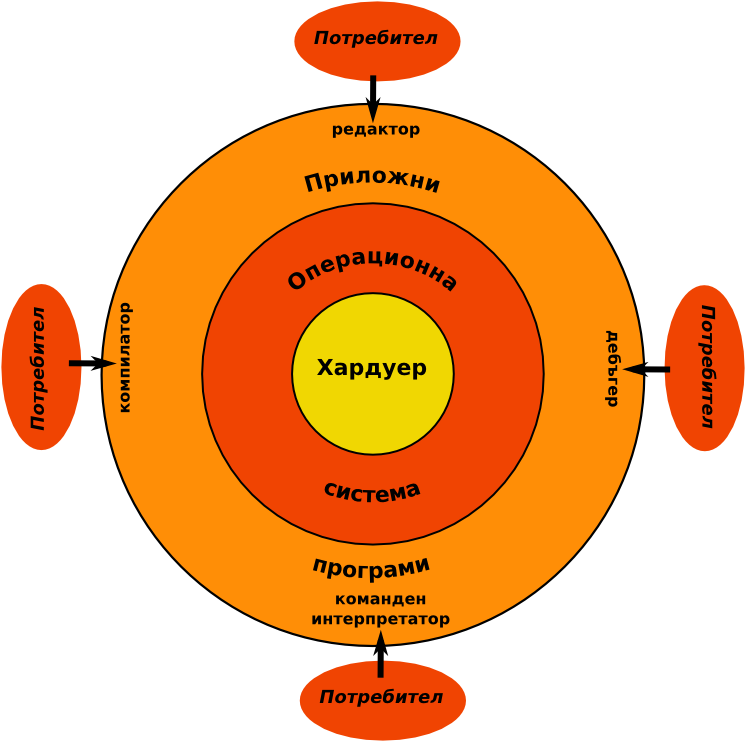
\includegraphics{pics/01-computer-structure}}
\caption{Обща структура на компютърна система}
\end{figure}
\end{frame}

%-------------------------------------------------------------------- SECTION -
\section{Основни елементи на компютърната система}

%---------------------------------------------------------------------- SLIDE -
\begin{frame}
\frametitle{Основни елементи на компютърна система}
\begin{itemize}
\item Централен процесор.
\item Оперативна памет.
\begin{itemize}
  \item Енергозависима.
\end{itemize}
\item Входно/изходни устройства.
\begin{itemize}
  \item Външни запаметяващи устройства.
  \item Комуникационни и мрежови устройства.
  \item Терминали.
\end{itemize}
\item Системна шина.
\begin{itemize}
  \item Осъществява връзката между процесора, паметта и входно/изходните
  устройства.
\end{itemize}
\end{itemize}
\end{frame}


%---------------------------------------------------------------------- SLIDE -
\begin{frame}
\frametitle{Структура на компютърна система}
\begin{figure}[h]
\center
\scalebox{0.4}{\includegraphics{pics/02-computer-system-structure}}
\caption{Структура на компютърна система}
\end{figure}
\end{frame}


%-------------------------------------------------------------------- SECTION -
\section{Централен процесор}

%---------------------------------------------------------------------- SLIDE -
\begin{frame}
\frametitle{Централен процесор}
\begin{itemize}
\item Процесорът изпълнява инструкциите на програмата.
\item Инструкциите на програмата и данните се съхраняват в оперативната памет.
\item Регистрите на процесора са високоскоростна памет, разположена в самия
процесор. 
\item Данните трябва да са в регистрите на процесора, за да може
{\em аритметико-логическия блок} да ги обработва. 
\item За да се изпълни дадена инструкция тя първо трябва да се {\em извлече (fetch)} и
{\em декодира (decode)}.
\end{itemize}
\end{frame}

%---------------------------------------------------------------------- SLIDE -
\begin{frame}
\frametitle{Централен процесор}
\begin{figure}[h]
\center
\scalebox{0.4}{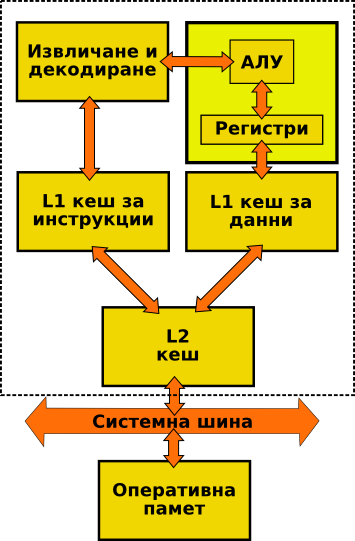
\includegraphics{pics/02-processor}}
\caption{Структура на компютърна система}
\end{figure}
\end{frame}


%---------------------------------------------------------------------- SLIDE -
\begin{frame}
\frametitle{Регистри на процесора}
\begin{itemize}
\item Регистри с общо предназначение.
\begin{itemize}
  \item Достъпни са за всички програми.
\end{itemize}
\item Контролни регистри.
\begin{itemize}
  \item Използват се от процесора за да контролират работата му.
  \item Използват се от операционната система за да контролират изпълнението на
  приложните програми.
\end{itemize}
\end{itemize}
\end{frame}

%---------------------------------------------------------------------- SLIDE -
\begin{frame}
\frametitle{Регистри с общо предназначение}
\begin{itemize}
\item Достъпни са за всички програми.
\item Могат да се адресират като се използва асемблер.
\item Има два типа:
\begin{itemize}
  \item Регистри за данни.
  \item Адресни регистри:
  \begin{itemize}
    \item Използват се за реализация на различни схеми за адресация.
    \item Индексен, сегментен, указател на стека.
  \end{itemize}
\end{itemize}
\end{itemize}
\end{frame}


%---------------------------------------------------------------------- SLIDE -
\begin{frame}
\frametitle{Контролни регистри}
\begin{itemize}
\item Не са достъпни директно.
\item Програмен брояч (Program Counter -- PC).
\begin{itemize}
  \item Съдържа адреса на следващата инструкция, която трябва да бъде извлечена.
\end{itemize}
\item Регистър за инструкция (Instruction Register -- IR).
\begin{itemize}
  \item Съдържа последната извлечена от паметта инструкция.
\end{itemize}
\item Регистър на състоянието (Program Status Word -- PSW).
\begin{itemize}
  \item Резултат от сравнения.
  \item Разрешаване и забрана на прекъсванията.
  \item Потребителски режим и защитен режим на процесора.
\end{itemize}
\end{itemize}
\end{frame}

%---------------------------------------------------------------------- SLIDE -
\begin{frame}
\frametitle{Извличане и изпълнение на инструкции}
\begin{itemize}
\item Процесорът извлича инструкции от оперативната памет.
\item Програмният брояч (PC) съдържа адреса на инструкцията, която трябва да
бъде извлечена.
\item След всяко извличане на инструкция, програмния брояч се увеличава.
\item Извлечената инструкция се съхранява в регистъра за инструкции.
\end{itemize}
\begin{figure}[h]
\center
\scalebox{0.4}{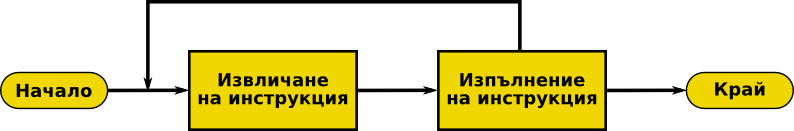
\includegraphics{pics/02-fetch-execute-cycle}}
\caption{Основен цикъл за изпълнение на инструкции}
\end{figure}
\end{frame}

%-------------------------------------------------------------------- SECTION -
\section{Входно/изходни устройства}

%----------------------------------------------------------------- SUBSECTION -
\subsection{Управление на периферните устройства}

%---------------------------------------------------------------------- SLIDE -
\begin{frame}
\frametitle{Управление на периферните устройства}
\begin{itemize}
\item Има няколко начина за управление на входно/изходните устройства от
процесора:
\begin{itemize}
  \item Синхронно изпълнение на входно/изходните операции (Programmed IO).
  \item Асинхронно изпълнение на входно/изходните операции (Interrupt-Driven IO).
  \item Пряк достъп до паметта (Direct Memory Access).
\end{itemize}
\end{itemize}
\end{frame}

%---------------------------------------------------------------------- SLIDE -
\begin{frame}
\frametitle{Синхронно изпълнение на IO}
\begin{columns}
\column{0.6\textwidth}
\begin{itemize}
\item Процесорът се обръща към контролера на входно/изходното устройство и
подава заявка за извършване на операцията.
\item Входно/изходната операция се извършва от контролера на устройството.
\item Процесора трябва постоянно проверява за състоянието на операцията, докато
тя завърши. 
\end{itemize}
\column{0.4\textwidth}
\begin{figure}[h]
\center
\scalebox{0.33}{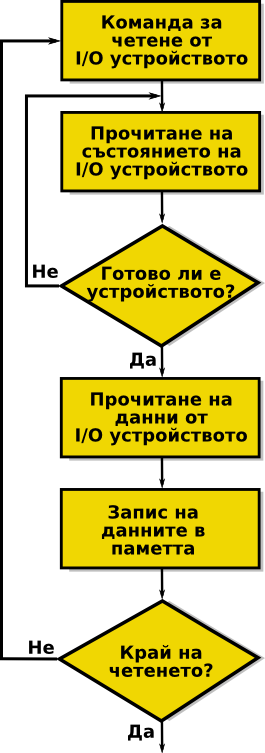
\includegraphics{pics/02-programmed-IO}}
\end{figure}
\end{columns}
\end{frame}


%---------------------------------------------------------------------- SLIDE -
\begin{frame}
\frametitle{Асинхронно изпълнение на IO}
\begin{columns}
\column{0.6\textwidth}
\begin{itemize}
\item Процесорът се обръща към контролера на входно/изходното устройство и
подава заявка за извършване на операцията.
\item След подаване на заявката, процесорът е свободен да се занимава с други
задачи.
\item Когато изпълнението на операцията завърши, контролерът на входно/изходното
устройство {\em прекъсва} работата на процесора.
\item Процесорът трябва да прехвърли данните от буферите на контролера в
оперативната памет или регистрите си.
\end{itemize}
\column{0.4\textwidth}
\begin{figure}[h]
\center
\scalebox{0.33}{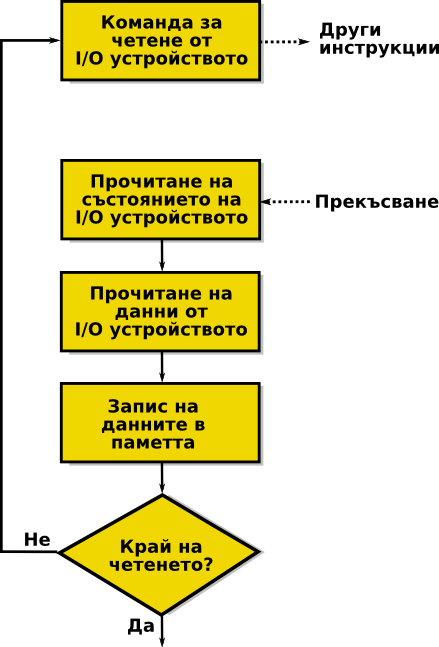
\includegraphics{pics/02-interrupt-IO}}
\end{figure}
\end{columns}
\end{frame}


%---------------------------------------------------------------------- SLIDE -
\begin{frame}
\frametitle{Пряк достъп до паметта}
\begin{columns}
\column{0.6\textwidth}
\begin{itemize}
\item Чете блокове от данни директно в оперативната памет.
\item Работата на процесора се прекъсва когато целият блок от данни е прочетен и
копиран в оперативната памет.
\item Процесорът не се занимава с копиране на данните от буфера на устройството
в оперативната памет.
\end{itemize}
\column{0.4\textwidth}
\begin{figure}[h]
\center
\scalebox{0.33}{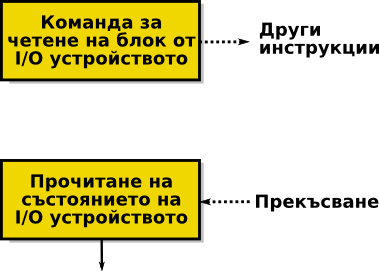
\includegraphics{pics/02-dma}}
\end{figure}
\end{columns}
\end{frame}


%----------------------------------------------------------------- SUBSECTION -
\subsection{Обработка на прекъсванията}

%---------------------------------------------------------------------- SLIDE -
\begin{frame}
\frametitle{Обработка на прекъсванията}
\begin{itemize}
\item Прекъсват нормалната последователност на изпълнение на команди от
процесора.
\item Прекъсването предава управлението на функцията за обработване на
прекъсването.
\item Прекъсването на обработваното задание става по такъв начин, че да е
възможно възстановяване на неговата обработка.
\item Операционната система запазва състоянието на процесора като запазва
регистрите, програмния брояч и т.н.
\item Определя какъв е видът на прекъсването и къде точно трябва да се
предаде управлението за да се обработи възникналото прекъсване.
\end{itemize}
\end{frame}

%---------------------------------------------------------------------- SLIDE -
\begin{frame}
\frametitle{Цикъл за обработка на прекъсванията}
\begin{figure}[h]
\center
\scalebox{0.4}{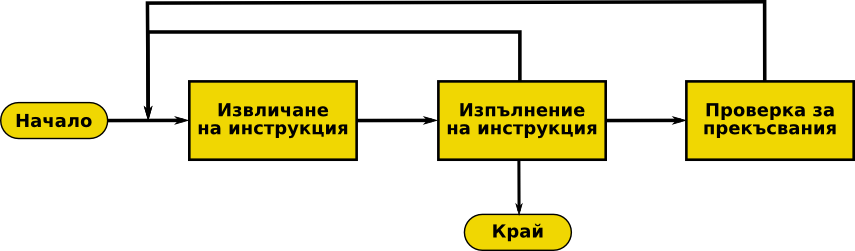
\includegraphics{pics/02-fetch-execute-interrupt-cycle}}
\caption{Цикъл за обработка на прекъсванията}
\end{figure}
\end{frame}



%---------------------------------------------------------------------- SLIDE -
\begin{frame}
\frametitle{Видове прекъсвания}
\begin{itemize}
\item Софтуерни прекъсвания (trap):
\begin{itemize}
  \item препълване при аритметични операции;
  \item делене на нула;
  \item изпълнение на неправилна инструкция;
  \item опит за достъп до защитена част от паметта.
\end{itemize}
\item Прекъсвания от таймера.
\item Прекъсвания от входно/изходните устройства.
\item Прекъсвания предизвикани от повреди в хардуера.
\end{itemize}
\end{frame}

%---------------------------------------------------------------------- SLIDE -
\begin{frame}
\frametitle{Обработка на много прекъсвания}
\begin{itemize}
\item Последователна обработка на множество прекъсвания:
\begin{itemize}
  \item Прекъсванията се забраняват докато процесорът не завърши обработката на
  текущото прекъсване.
  \item Възникналите нови прекъсвания чакат процесора да разреши обработката на
  прекъсвания.
  \item След като функцията за обработка на прекъсването завърши, процесорът
  проверява за нови прекъсвания.
\end{itemize}
\item Обработка на множество прекъсвания с приоритети.
\begin{itemize}
  \item Прекъсванията с по-висок приоритет могат да предизвикат прекъсване на
  функцията за обработка на прекъсвания с по-нисък приоритет.
\end{itemize}
\end{itemize}
\end{frame}

%---------------------------------------------------------------------- SLIDE -
\begin{frame}
\frametitle{Пряк достъп до паметта (DMA)}
\begin{itemize}
\item Прекият достъп до паметта съществено подобрява скоростта на трансфер на
данни между входно/изходните устройства и оперативната памет.
\item Типично прекият достъп до паметта (DMA) се използва от бързи входно
изходни устройства -- твърди дискове, мрежови контролери и т.н.
\item Контролерът на устройството прехвърля блок от данни директно в/от оперативната
памет без намеса на централния процесор.
\item Генерира се само едно прекъсване за целия блок от данни.
\end{itemize}
\end{frame}

%-------------------------------------------------------------------- SECTION -
\section{Памет}


%---------------------------------------------------------------------- SLIDE -
\begin{frame}
\frametitle{Памет}
\begin{itemize}
\item Оперативна памет.
\begin{itemize}
  \item Процесора може да работи директно с оперативната памет.
  \item Типично оперативната памет е енергозависима.
  \item Процесорът има достъп до клетките на паметта в произволен ред.
\end{itemize}
\item Външни запомнящи устройства.
\begin{itemize}
  \item Може да съхраняват по-големи обеми от данни при по-ниска цена.
  \item Енергонезависима памет.
  \item Скоростта на достъп до данните типично е с порядъци по-малка.
\end{itemize}
\end{itemize}
\end{frame}

%---------------------------------------------------------------------- SLIDE -
\begin{frame}
\frametitle{Йерархия на паметта}
\begin{figure}[h]
\center
\scalebox{0.7}{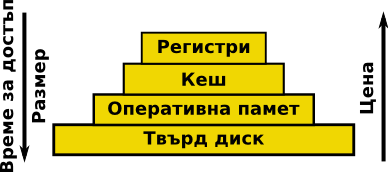
\includegraphics{pics/02-memory-hierarchy}}
\caption{Йерархия на паметта}
\end{figure}
\end{frame}


%---------------------------------------------------------------------- SLIDE -
\begin{frame}
\frametitle{Кеширане}
\begin{itemize}
\item Важен принцип, който се реализира на различни нива в компютърната система
(на хардуерно ниво, в операционната система, в приложните програми).
\item Използваната информация временно се копира от по-бавно в по-бързо
запомнящо устройство.
\item Когато има нужда от дадена информация, първо се проверява кеша.
\begin{itemize}
  \item Ако нужната информация е налична в кеша, то директно се използва тя.
  \item Ако не, информацията първо се копира в кеша, и след това се чете от там.
\end{itemize}
\item Кешът е по-малък от паметта, която се кешира.
\begin{itemize}
  \item Политика за управление на кеша.
  \item Политика за обновяване на кеша.
\end{itemize} 
\end{itemize}
\end{frame}


%-------------------------------------------------------------------- SECTION -
\section{Хардуерна поддръжка на операционната система}


%---------------------------------------------------------------------- SLIDE -
\begin{frame}
\frametitle{Хардуерна поддръжка на ОС}
\begin{itemize}
\item Компютърните системи съдържат хардуерни механизми, които:
\begin{itemize}
  \item позволяват на операционната система да изпълнява основните си функции
  бързо;
  \item  позволяват на операционната система стриктно да прилага механизми за
  защита на информацията. 
\end{itemize}
\item Основните механизми за защита, използвани в компютърните системи са:
\begin{itemize}
  \item Два режима на работа на процесора.
  \item Защита на входно/изходните операции.
  \item Защита на паметта.
  \item Защита на централния процесор.
\end{itemize}
\item Механизмите за защита използвани от операционната система типично се
  реализират в централния процесор.
\end{itemize}
\end{frame}


%---------------------------------------------------------------------- SLIDE -
\begin{frame}
\frametitle{Два режима на процесора}
\begin{itemize}
  \item Поделянето на ресурсите на операционната система изисква изграждането на
  механизми,
  които да не позволяват на некоректно работеща програма да наруши правилната
  работа на другите програми.
  \item Хардуерно в централния процесор типично се реализират поне  два режима на
  работа:
  \begin{itemize}
    \item Потребителски режим -- в този режим може да се изпълнява само
    подмножество от инструкции на процесора, които се считат за безопасни. 
    Режимът в който работят потребителските програми.
    \item Режим на ядрото (привилегирован режим, защитен режим) -- могат да се
    изпълняват всички инструкции на процесора. Режимът в който работи
    операционната система.
  \end{itemize}
  \item В регистъра за състоянието на процесора (PSW) се добавя бит, който да
  показва какъв е режимът на работа на процесора.
  \item При възникване на прекъсване процесорът преминава в защитен режим.

\end{itemize}

\end{frame}


%---------------------------------------------------------------------- SLIDE -
\begin{frame}
\frametitle{Защита на входно/изходните операции и прекъсвания}
\begin{itemize}
\item Не бива да позволява на потребителската програма да получи контрол
върху процесора в привилегирован режим.
\item Всички инструкции за изпълнение на входно/изходни операции се
изпълняват само в привилегирован режим на процесора.

\item Прекъсвания
\begin{itemize}
    \item Повечето входно/изходни устройства изпращат прекъсване на процесора в
    случай, че настъпи някакво събитие -- приключване на входно/изходна операция
    или хардуерна грешка.
    \item При обработване на прекъсване процесорът се превключва в
    привилегирован (защитен) режим.
    \item Обработването на прекъсването е работа на операционната система.
\end{itemize}
\end{itemize}
\end{frame}


%---------------------------------------------------------------------- SLIDE -
\begin{frame}
\frametitle{Защита и управление на паметта}
\begin{itemize}
\item Не позволява на процесите достъп до участъците от паметта, които не
принадлежат на тях.
\item Задължително е да се предостави защита на паметта за вектора на
прекъсванията и функциите за обработка на прекъсванията.
\item Реализира се чрез регистри на процесора, които могат да се променят
    само в защитен режим (привилегирован режим).
\item Добавят се два регистъра, които определят областта от паметта, която
програмата може да използва:
\begin{itemize}
  \item Базов регистър (base register) -- съдържа най-малкия адрес в паметта,
  който е достъпен (разрешен).
  \item Граничен регистър (limit register) -- съдържа размера на разрешения за
  използване участък от паметта.
\end{itemize}
\item Паметта, която е извън така дефинирания участък е защитена -- докато е в
потребителски режим процесорът няма достъп до нея.
% \item Инструкциите за промяна на съдържанието на тези адресни регистри могат да
% се изпълняват само в привилегирован режим.
\end{itemize}
\end{frame}

%---------------------------------------------------------------------- SLIDE -
\begin{frame}
\frametitle{Защита на паметта}
\begin{figure}[h]
\center
\scalebox{0.5}{\includegraphics{pics/02-memory-protection}}
\end{figure}
\end{frame}

%---------------------------------------------------------------------- SLIDE -
\begin{frame}
\frametitle{Защита на паметта}
\begin{figure}[h]
\center
\scalebox{0.45}{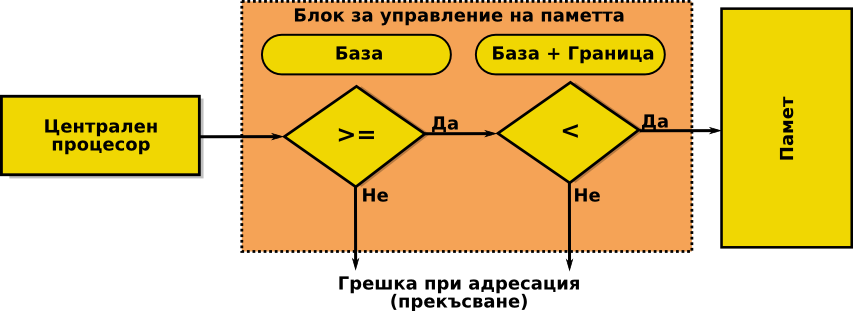
\includegraphics{pics/02-memory-protection-algo}}
\end{figure}
\end{frame}

%---------------------------------------------------------------------- SLIDE -
\begin{frame}
\frametitle{Защита на процесора: таймери}
\begin{itemize}
\item Таймерите генерират прекъсване към процесора след изтичането на определен
период от време.
\item Операционната система използва таймерите за да се защитава от процеси,
които монополизират използването на процесора.
\item Таймерите се използват при реализация на времеделене.
\item Задаването на таймер е привилегирована инструкция.
\end{itemize}
\end{frame}


\end{document}
